% ===========================================================================
%  TikuOS — TikuKits ML: Tiny Neural Network for Embedded Systems
%  Beamer Presentation
% ===========================================================================
\documentclass[aspectratio=169, 10pt]{beamer}

% ---- Theme ----------------------------------------------------------------
\usetheme{Madrid}
\usecolortheme{whale}
\setbeamertemplate{navigation symbols}{}
\setbeamertemplate{footline}{%
  \leavevmode\hbox{%
    \begin{beamercolorbox}[wd=.33\paperwidth,ht=2.5ex,dp=1ex,center]{author in head/foot}%
      \usebeamerfont{author in head/foot}\insertshortauthor
    \end{beamercolorbox}%
    \begin{beamercolorbox}[wd=.34\paperwidth,ht=2.5ex,dp=1ex,center]{title in head/foot}%
      \usebeamerfont{title in head/foot}\insertshorttitle
    \end{beamercolorbox}%
    \begin{beamercolorbox}[wd=.33\paperwidth,ht=2.5ex,dp=1ex,right]{date in head/foot}%
      \usebeamerfont{date in head/foot}\insertshortdate{}\hspace*{2em}%
      \insertframenumber{}/\inserttotalframenumber\hspace*{2ex}
    \end{beamercolorbox}}%
  \vskip0pt%
}

% ---- Packages -------------------------------------------------------------
\usepackage{listings}
\usepackage{graphicx}
\usepackage{hyperref}
\usepackage{booktabs}
\usepackage{multirow}
\usepackage{tikz}
\usetikzlibrary{arrows.meta, positioning, shapes.geometric, calc,
                decorations.pathreplacing, fit}
\usepackage{amsmath}

% ---- Code listing style ---------------------------------------------------
\lstset{
  basicstyle=\ttfamily\scriptsize,
  keywordstyle=\color{blue}\bfseries,
  commentstyle=\color{gray},
  stringstyle=\color{red!70!black},
  showstringspaces=false,
  breaklines=true,
  frame=single,
  rulecolor=\color{black!30},
  backgroundcolor=\color{blue!3},
  tabsize=4,
}
\lstdefinestyle{cstyle}{
  language=C,
  morekeywords={uint8_t,uint16_t,uint32_t,int32_t,int64_t,
                tiku_kits_ml_elem_t,
                TIKU_KITS_ML_OK,TIKU_KITS_ML_ERR_NULL,
                TIKU_KITS_ML_ERR_SIZE,TIKU_KITS_ML_ERR_PARAM,
                TIKU_KITS_ML_TNN_MAX_INPUT,
                TIKU_KITS_ML_TNN_MAX_HIDDEN,
                TIKU_KITS_ML_TNN_MAX_OUTPUT,
                TIKU_KITS_ML_TNN_SHIFT,
                NULL},
}

% ---- Metadata -------------------------------------------------------------
\title[TikuKits ML]{TikuKits ML: Tiny Neural Network for Embedded Systems}
\subtitle{Simple. Ubiquitous. Intelligence, Everywhere.}
\author[Ambuj Varshney]{Ambuj Varshney \\ \texttt{ambuj@tiku-os.org}}
\date{\today}

% ===========================================================================
\begin{document}

% ---------------------------------------------------------------------------
\begin{frame}
\titlepage
\end{frame}

% ---------------------------------------------------------------------------
\begin{frame}{Outline}
\tableofcontents
\end{frame}

% ===========================================================================
\section{Motivation}
% ===========================================================================

\begin{frame}{Why Neural Networks on MCUs?}
\begin{columns}[T]
\begin{column}{0.48\textwidth}
\begin{block}{Embedded Use Cases}
\begin{itemize}
  \item \textbf{Non-linear boundaries} --- what linear models cannot solve
  \item \textbf{Multi-class} --- temperature zones, gesture types
  \item \textbf{On-device training} --- adapt to local conditions
  \item \textbf{Universal approximation} --- learn any mapping
\end{itemize}
\end{block}

\begin{block}{Constraints}
\begin{itemize}
  \item No FPU (16-bit MSP430)
  \item No heap allocation
  \item 320-byte stack on MSP430
  \item Every $\mu$J counts
\end{itemize}
\end{block}
\end{column}

\begin{column}{0.48\textwidth}
\begin{center}
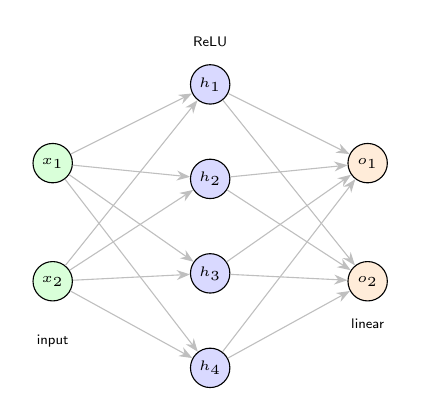
\begin{tikzpicture}[
    >=Stealth, node distance=0.4cm,
    neuron/.style={draw, circle, minimum size=0.5cm,
                   font=\tiny\sffamily, inner sep=0pt}
  ]
  % Input layer
  \node[neuron, fill=green!15] (i1) at (0, 2) {$x_1$};
  \node[neuron, fill=green!15] (i2) at (0, 0.5) {$x_2$};

  % Hidden layer
  \node[neuron, fill=blue!15] (h1) at (2, 3) {$h_1$};
  \node[neuron, fill=blue!15] (h2) at (2, 1.8) {$h_2$};
  \node[neuron, fill=blue!15] (h3) at (2, 0.6) {$h_3$};
  \node[neuron, fill=blue!15] (h4) at (2, -0.6) {$h_4$};

  % Output layer
  \node[neuron, fill=orange!15] (o1) at (4, 2) {$o_1$};
  \node[neuron, fill=orange!15] (o2) at (4, 0.5) {$o_2$};

  % Connections
  \foreach \i in {i1,i2} {
    \foreach \h in {h1,h2,h3,h4} {
      \draw[->, thin, gray!50] (\i) -- (\h);
    }
  }
  \foreach \h in {h1,h2,h3,h4} {
    \foreach \o in {o1,o2} {
      \draw[->, thin, gray!50] (\h) -- (\o);
    }
  }

  % Labels
  \node[font=\tiny\sffamily, above=0.1cm of h1] {ReLU};
  \node[font=\tiny\sffamily, below=0.1cm of o2] {linear};
  \node[font=\tiny\sffamily, below=0.3cm of i2] {input};
\end{tikzpicture}
\end{center}

\vspace{0.3em}
\begin{alertblock}{Design Goal}
Single-hidden-layer MLP with \textbf{ReLU activation},
\textbf{backpropagation}, and all computation in
integer fixed-point arithmetic.
\end{alertblock}
\end{column}
\end{columns}
\end{frame}

% ===========================================================================
\section{Algorithm Theory}
% ===========================================================================

\begin{frame}{Feedforward Neural Network}
\begin{columns}[T]
\begin{column}{0.48\textwidth}
\textbf{Forward pass:}

\vspace{0.3em}
Hidden layer (ReLU activation):
\[
  h_j = \text{ReLU}\!\left(w^h_{j,0} + \sum_{i=1}^{n} w^h_{j,i} \cdot x_i\right)
\]
where $\text{ReLU}(z) = \max(0, z)$.

\vspace{0.3em}
Output layer (linear):
\[
  o_k = w^o_{k,0} + \sum_{j=1}^{m} \frac{w^o_{k,j} \cdot h_j}{2^{\text{shift}}}
\]

\vspace{0.3em}
\textbf{Prediction:} $\hat{y} = \arg\max_k\; o_k$

\vspace{0.5em}
\textbf{Target:} One-hot encoding\\
$t_k = 2^{\text{shift}}$ if $k = y$, else $0$.
\end{column}

\begin{column}{0.48\textwidth}
\textbf{Backpropagation (SGD):}

\vspace{0.3em}
Output error:
\[
  \delta^o_k = o_k - t_k
\]

Hidden error (uses \textbf{old} output weights):
\[
  \delta^h_j = \begin{cases}
    \sum_k \frac{w^o_{k,j+1} \cdot \delta^o_k}{2^{\text{shift}}} & \text{if } h_j > 0\\
    0 & \text{otherwise}
  \end{cases}
\]

\vspace{0.3em}
\begin{alertblock}{Critical: Update Order}
Hidden weights must be updated \textbf{before}
output weights --- otherwise, error propagation
uses modified weights and learning fails.
\end{alertblock}
\end{column}
\end{columns}
\end{frame}

% ---------------------------------------------------------------------------
\begin{frame}{Why ReLU for Embedded?}
\begin{columns}[T]
\begin{column}{0.48\textwidth}
\begin{center}
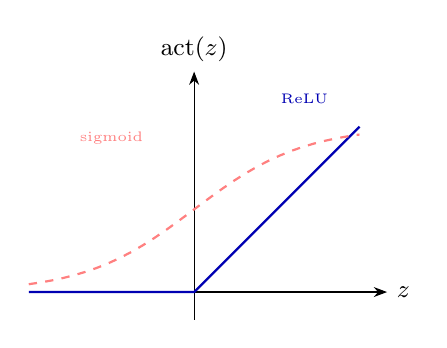
\begin{tikzpicture}[>=Stealth, scale=0.7]
  % Axes
  \draw[->] (-3,0) -- (3.5,0) node[right] {\small $z$};
  \draw[->] (0,-0.5) -- (0,4) node[above] {\small $\text{act}(z)$};

  % ReLU
  \draw[thick, blue!70!black] (-3, 0) -- (0, 0) -- (3, 3);

  % Sigmoid (approximate)
  \draw[thick, red!50, dashed, domain=-3:3, samples=30]
    plot (\x, {3/(1+exp(-\x))});

  % Labels
  \node[font=\tiny, blue!70!black] at (2, 3.5) {ReLU};
  \node[font=\tiny, red!50] at (-1.5, 2.8) {sigmoid};
\end{tikzpicture}
\end{center}
\end{column}

\begin{column}{0.48\textwidth}
\begin{block}{ReLU Advantages for MCU}
\begin{enumerate}
  \item \textbf{No transcendentals:}\\
    $\text{ReLU}(z) = \max(0, z)$\\
    One comparison, no \texttt{exp()}.
  \item \textbf{Integer-friendly derivative:}\\
    $\text{ReLU}'(z) = \begin{cases} 1 & z > 0 \\ 0 & z \leq 0 \end{cases}$
  \item \textbf{No saturation:}\\
    Positive values pass through unchanged.
  \item \textbf{Sparse activation:}\\
    Negative inputs produce zero --- less work.
\end{enumerate}
\end{block}
\end{column}
\end{columns}
\end{frame}

% ===========================================================================
\section{Data Structure}
% ===========================================================================

\begin{frame}[fragile]{The \texttt{tiku\_kits\_ml\_tnn} Structure}
\begin{columns}[T]
\begin{column}{0.48\textwidth}
\begin{lstlisting}[style=cstyle,
  title={ml/classification/tiku\_kits\_ml\_tnn.h}]
struct tiku_kits_ml_tnn {
    /* Hidden weights: [hidden][input+1] */
    int32_t w_hidden
        [TIKU_KITS_ML_TNN_MAX_HIDDEN]
        [TIKU_KITS_ML_TNN_MAX_INPUT + 1];
    /* Output weights: [output][hidden+1] */
    int32_t w_output
        [TIKU_KITS_ML_TNN_MAX_OUTPUT]
        [TIKU_KITS_ML_TNN_MAX_HIDDEN + 1];
    /* Scratch: activations */
    int32_t h[TIKU_KITS_ML_TNN_MAX_HIDDEN];
    int32_t o[TIKU_KITS_ML_TNN_MAX_OUTPUT];

    uint8_t  n_input, n_hidden, n_output;
    uint8_t  shift;
    int32_t  learning_rate;
    uint16_t n;
};
\end{lstlisting}
\end{column}

\begin{column}{0.48\textwidth}
\begin{lstlisting}[style=cstyle,
  title={Configuration macros}]
#ifndef TIKU_KITS_ML_TNN_MAX_INPUT
#define TIKU_KITS_ML_TNN_MAX_INPUT  8
#endif
#ifndef TIKU_KITS_ML_TNN_MAX_HIDDEN
#define TIKU_KITS_ML_TNN_MAX_HIDDEN 8
#endif
#ifndef TIKU_KITS_ML_TNN_MAX_OUTPUT
#define TIKU_KITS_ML_TNN_MAX_OUTPUT 4
#endif
\end{lstlisting}

\textbf{Memory footprint:}\\
$8 \times 9 \times 4 + 4 \times 9 \times 4 + 8 \times 4 + 4 \times 4 + 10$\\
$= 442$ bytes (default config).

\vspace{0.3em}
\begin{block}{Stack Safety}
Scratch buffers \texttt{h[]} and \texttt{o[]} are stored
\textbf{in the struct}, not on the stack --- critical for
MSP430's 320-byte stack limit.
\end{block}
\end{column}
\end{columns}
\end{frame}

% ===========================================================================
\section{API Reference}
% ===========================================================================

\begin{frame}[fragile]{Complete API}
\begin{table}
\centering
\small
\begin{tabular}{@{}lp{8cm}@{}}
\toprule
\textbf{Function} & \textbf{Description} \\
\midrule
\texttt{tiku\_kits\_ml\_tnn\_init(tnn, ni, nh, no, sh)}
  & Initialize with \texttt{ni} inputs, \texttt{nh} hidden, \texttt{no} outputs \\
\texttt{tiku\_kits\_ml\_tnn\_reset(tnn)}
  & Reinitialize weights, reset training count \\
\texttt{tiku\_kits\_ml\_tnn\_set\_lr(tnn, rate)}
  & Set learning rate in Q(shift) \\
\midrule
\texttt{tiku\_kits\_ml\_tnn\_train(tnn, x, y)}
  & One backpropagation SGD step; label $y \in [0, \text{n\_output})$ \\
\texttt{tiku\_kits\_ml\_tnn\_predict(tnn, x, \&result)}
  & Forward pass + argmax: returns predicted class \\
\texttt{tiku\_kits\_ml\_tnn\_forward(tnn, x, scores)}
  & Forward pass only: returns all output scores \\
\midrule
\texttt{tiku\_kits\_ml\_tnn\_get\_weights(tnn, layer, w)}
  & Export weights (layer 0=hidden, 1=output) \\
\texttt{tiku\_kits\_ml\_tnn\_set\_weights(tnn, layer, w)}
  & Load pre-trained weights \\
\texttt{tiku\_kits\_ml\_tnn\_count(tnn)}
  & Number of training samples seen \\
\bottomrule
\end{tabular}
\end{table}

\vspace{0.3em}
\begin{alertblock}{Minimum Classes}
\texttt{init()} requires $\text{n\_output} \geq 2$ (classification needs at least 2 classes).
Default learning rate: $(1 \ll \text{shift}) / 20 \approx 0.05$ in Q8 $= 12$.
\end{alertblock}
\end{frame}

% ===========================================================================
\section{Implementation Details}
% ===========================================================================

\begin{frame}[fragile]{Weight Initialization}
\begin{columns}[T]
\begin{column}{0.48\textwidth}
\begin{lstlisting}[style=cstyle,
  title={Symmetry-breaking initialization}]
static void init_weights(
    struct tiku_kits_ml_tnn *tnn)
{
    uint8_t j, i, k;
    int32_t scale;

    /* ~1/n_input in Q(shift) */
    scale = (int32_t)(
        (1 << tnn->shift)
        / (tnn->n_input + 1));
    if (scale < 1) scale = 1;

    /* Hidden: alternating +/- scale */
    for (j = 0; j < tnn->n_hidden; j++) {
        tnn->w_hidden[j][0] = 0; /* bias */
        for (i = 1; i <= tnn->n_input; i++){
            tnn->w_hidden[j][i] =
                ((j + i) & 1)
                    ? scale : -scale;
        }
    }

    /* Output: all zero */
    for (k = 0; k < tnn->n_output; k++)
        for (j = 0; j <= tnn->n_hidden; j++)
            tnn->w_output[k][j] = 0;
}
\end{lstlisting}
\end{column}

\begin{column}{0.48\textwidth}
\begin{block}{Why Alternating Signs?}
\begin{itemize}
  \item If all hidden weights are identical, all neurons
    compute the same function --- \textbf{symmetry problem}
  \item Alternating $\pm$ ensures different neurons
    respond to different aspects of the input
  \item Scale $\approx 1/n$ prevents initial saturation
  \item No randomness needed (deterministic, reproducible)
\end{itemize}
\end{block}

\vspace{0.3em}
\begin{block}{Output Layer: All Zeros}
Output weights start at zero so all classes begin
with equal score. The network learns to differentiate
through backpropagation.
\end{block}
\end{column}
\end{columns}
\end{frame}

% ---------------------------------------------------------------------------
\begin{frame}[fragile]{Forward Pass and Backpropagation}
\begin{columns}[T]
\begin{column}{0.48\textwidth}
\begin{lstlisting}[style=cstyle,
  title={Forward pass (hidden + output)}]
/* Hidden layer: ReLU */
for (j = 0; j < tnn->n_hidden; j++) {
    acc = (int64_t)tnn->w_hidden[j][0];
    for (i = 0; i < tnn->n_input; i++) {
        acc += (int64_t)tnn->w_hidden[j][i+1]
               * (int64_t)x[i];
    }
    tnn->h[j] = (acc > 0)
        ? (int32_t)acc : 0;
}

/* Output layer: linear */
for (k = 0; k < tnn->n_output; k++) {
    acc = (int64_t)tnn->w_output[k][0];
    for (j = 0; j < tnn->n_hidden; j++) {
        acc += ((int64_t)tnn->w_output[k][j+1]
                * (int64_t)tnn->h[j])
               >> tnn->shift;
    }
    tnn->o[k] = (int32_t)acc;
}
\end{lstlisting}
\end{column}

\begin{column}{0.48\textwidth}
\begin{lstlisting}[style=cstyle,
  title={Backprop: hidden FIRST, then output}]
/* 1. Hidden gradients (old output wts) */
for (j = 0; j < tnn->n_hidden; j++) {
    if (tnn->h[j] <= 0) continue;
    err_sum = 0;
    for (k = 0; k < tnn->n_output; k++) {
        delta_o = tnn->o[k]
            - ((k == y) ? one_q : 0);
        err_sum += ((int64_t)
            tnn->w_output[k][j + 1]
            * (int64_t)delta_o)
            >> tnn->shift;
    }
    /* Update hidden weights */
    lr_delta = (lr_q * err_sum)
               >> tnn->shift;
    tnn->w_hidden[j][0] -= lr_delta;
    for (i = 0; i < tnn->n_input; i++)
        tnn->w_hidden[j][i+1] -=
            lr_delta * (int64_t)x[i];
}

/* 2. Output weights (safe to update) */
for (k = 0; k < tnn->n_output; k++) {
    delta_o = tnn->o[k]
        - ((k == y) ? one_q : 0);
    /* ... update output weights ... */
}
\end{lstlisting}
\end{column}
\end{columns}
\end{frame}

% ===========================================================================
\section{Fixed-Point Details}
% ===========================================================================

\begin{frame}{Fixed-Point Arithmetic in the Network}
\begin{columns}[T]
\begin{column}{0.48\textwidth}
\begin{block}{Q-Format Flow}
\begin{itemize}
  \item \textbf{Inputs:} Integer scale (raw sensor values)
  \item \textbf{Hidden weights:} Q(shift)
  \item \textbf{Hidden activations:} $w \times x$ = Q(shift)
  \item \textbf{Output weights:} Q(shift)
  \item \textbf{Output products:} $w^o \times h = $ Q(2$\times$shift)\\
    $\rightarrow$ right-shift by \texttt{shift} to get Q(shift)
  \item \textbf{Targets:} $1 \ll \text{shift}$ (one-hot in Q(shift))
\end{itemize}
\end{block}
\end{column}

\begin{column}{0.48\textwidth}
\begin{block}{Overflow Prevention}
\begin{itemize}
  \item All products computed as \texttt{int64\_t}
  \item $\text{int32} \times \text{int32} = \text{int64}$
  \item Two-step \texttt{lr\_delta} avoids triple products:
    \begin{enumerate}
      \item $\text{lr\_delta} = (\eta \times \delta) \gg \text{shift}$
      \item $w \mathrel{-}= \text{lr\_delta} \times x$
    \end{enumerate}
  \item Safe for 8 inputs, 8 hidden, 4 outputs
\end{itemize}
\end{block}

\vspace{0.3em}
\begin{block}{Default Learning Rate}
$(1 \ll 8) / 20 = 12 \approx 0.047$ in Q8.\\
Typical range: 6--25 (0.025--0.1).
\end{block}
\end{column}
\end{columns}
\end{frame}

% ===========================================================================
\section{Examples}
% ===========================================================================

\begin{frame}[fragile]{Example 1: Temperature Zone Classification}
\begin{lstlisting}[style=cstyle,
  title={examples/example\_ml\_tnn.c --- 1 input, 3 output classes}]
struct tiku_kits_ml_tnn tnn;
uint8_t result;

/* 1 input, 4 hidden, 3 outputs, Q8 */
tiku_kits_ml_tnn_init(&tnn, 1, 4, 3, 8);
tiku_kits_ml_tnn_set_lr(&tnn, 6);   /* ~0.025 */

/* Training data: cold=0, normal=1, hot=2 */
static const int32_t temps[] = {50, 100, 150, 200, 250, 300, 350, 400, 450};
static const uint8_t labels[] = { 0,   0,   0,   1,   1,   1,   2,   2,   2};

uint16_t epoch;
uint8_t s;
for (epoch = 0; epoch < 80; epoch++) {
    for (s = 0; s < 9; s++) {
        tiku_kits_ml_tnn_train(&tnn, &temps[s], labels[s]);
    }
}

/* Predict */
int32_t query = 120;
tiku_kits_ml_tnn_predict(&tnn, &query, &result);  /* result = 0 (cold) */

query = 260;
tiku_kits_ml_tnn_predict(&tnn, &query, &result);  /* result = 1 (normal) */

query = 420;
tiku_kits_ml_tnn_predict(&tnn, &query, &result);  /* result = 2 (hot) */
\end{lstlisting}
\end{frame}

% ---------------------------------------------------------------------------
\begin{frame}[fragile]{Example 2: Gesture Recognition}
\begin{columns}[T]
\begin{column}{0.52\textwidth}
\begin{lstlisting}[style=cstyle,
  title={2-D accel: push vs. pull}]
struct tiku_kits_ml_tnn tnn;
uint8_t result;
int32_t scores[2];

/* 2 inputs, 4 hidden, 2 outputs, Q8 */
tiku_kits_ml_tnn_init(&tnn, 2, 4, 2, 8);
tiku_kits_ml_tnn_set_lr(&tnn, 13);

/* Push (class 0): +X, small Y */
tiku_kits_ml_elem_t push1[] = {10, 2};
tiku_kits_ml_elem_t push2[] = {12, -1};

/* Pull (class 1): -X, small Y */
tiku_kits_ml_elem_t pull1[] = {-10, 1};
tiku_kits_ml_elem_t pull2[] = {-8, -2};

/* Train 50 epochs */
uint16_t ep;
for (ep = 0; ep < 50; ep++) {
    tiku_kits_ml_tnn_train(&tnn, push1, 0);
    tiku_kits_ml_tnn_train(&tnn, push2, 0);
    tiku_kits_ml_tnn_train(&tnn, pull1, 1);
    tiku_kits_ml_tnn_train(&tnn, pull2, 1);
}

/* Classify + get scores */
tiku_kits_ml_elem_t q[] = {8, 0};
tiku_kits_ml_tnn_predict(&tnn, q, &result);
tiku_kits_ml_tnn_forward(&tnn, q, scores);
\end{lstlisting}
\end{column}

\begin{column}{0.44\textwidth}
\begin{center}
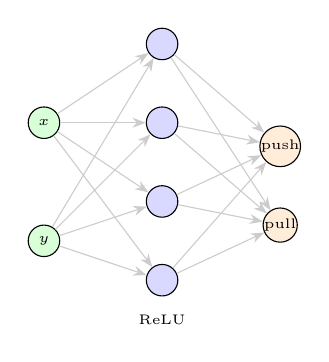
\begin{tikzpicture}[
    >=Stealth, node distance=0.3cm,
    neuron/.style={draw, circle, minimum size=0.4cm,
                   font=\tiny, inner sep=0pt}
  ]
  % Input
  \node[neuron, fill=green!15] (x1) at (0, 1.5) {$x$};
  \node[neuron, fill=green!15] (x2) at (0, 0) {$y$};

  % Hidden
  \node[neuron, fill=blue!15] (h1) at (1.5, 2.5) {};
  \node[neuron, fill=blue!15] (h2) at (1.5, 1.5) {};
  \node[neuron, fill=blue!15] (h3) at (1.5, 0.5) {};
  \node[neuron, fill=blue!15] (h4) at (1.5, -0.5) {};

  % Output
  \node[neuron, fill=orange!15] (o1) at (3, 1.2) {push};
  \node[neuron, fill=orange!15] (o2) at (3, 0.2) {pull};

  \foreach \i in {x1,x2} \foreach \h in {h1,h2,h3,h4}
    \draw[->, thin, gray!40] (\i) -- (\h);
  \foreach \h in {h1,h2,h3,h4} \foreach \o in {o1,o2}
    \draw[->, thin, gray!40] (\h) -- (\o);

  \node[font=\tiny] at (1.5, -1.0) {ReLU};
\end{tikzpicture}
\end{center}

\vspace{0.5em}
\begin{block}{Raw Scores via \texttt{forward()}}
\texttt{tnn\_forward()} returns per-class output
scores in Q(shift). Higher score = more likely.
Use for:
\begin{itemize}
  \item Confidence thresholding
  \item Score-based triage
  \item Multi-output comparison
\end{itemize}
\end{block}
\end{column}
\end{columns}
\end{frame}

% ---------------------------------------------------------------------------
\begin{frame}[fragile]{Example 3: Pre-Trained Deployment}
\begin{lstlisting}[style=cstyle,
  title={Load weights trained offline}]
struct tiku_kits_ml_tnn tnn;
uint8_t result;

tiku_kits_ml_tnn_init(&tnn, 1, 2, 2, 8);

/* Hidden layer: 2 neurons x (1 bias + 1 input) = 4 weights */
int32_t w_hidden[] = {
    0,  256,     /* neuron 0: ReLU(x)   */
    0, -256,     /* neuron 1: ReLU(-x)  */
};
tiku_kits_ml_tnn_set_weights(&tnn, 0, w_hidden);

/* Output layer: 2 classes x (1 bias + 2 hidden) = 6 weights */
int32_t w_output[] = {
    0,  256,    0,     /* class 0: high when ReLU(x) > 0  (x > 0) */
    0,    0,  256,     /* class 1: high when ReLU(-x) > 0 (x < 0) */
};
tiku_kits_ml_tnn_set_weights(&tnn, 1, w_output);

/* Predict */
int32_t pos = 5;
tiku_kits_ml_tnn_predict(&tnn, &pos, &result);    /* result = 0 */

int32_t neg = -5;
tiku_kits_ml_tnn_predict(&tnn, &neg, &result);    /* result = 1 */
\end{lstlisting}
\end{frame}

% ===========================================================================
\section{Test Suite}
% ===========================================================================

\begin{frame}{Test Cases Overview}
\begin{table}
\centering
\small
\begin{tabular}{@{}clp{7cm}@{}}
\toprule
\textbf{\#} & \textbf{Test Function} & \textbf{What It Verifies} \\
\midrule
1 & \texttt{test\_kits\_ml\_tnn\_init}
  & Initialization, parameter bounds, n\_output $\geq 2$ \\
2 & \texttt{test\_kits\_ml\_tnn\_pretrained}
  & Hand-crafted weights: ReLU(x) vs ReLU(-x) \\
3 & \texttt{test\_kits\_ml\_tnn\_forward\_pass}
  & Raw output scores match expected values \\
4 & \texttt{test\_kits\_ml\_tnn\_training}
  & 2-input, 4-hidden, 2-output convergence (50 epochs) \\
5 & \texttt{test\_kits\_ml\_tnn\_three\_class}
  & 1-input, 4-hidden, 3-output convergence (80 epochs) \\
6 & \texttt{test\_kits\_ml\_tnn\_learning\_rate}
  & Custom learning rate accepted \\
7 & \texttt{test\_kits\_ml\_tnn\_weight\_access}
  & Get/set weights round-trip (both layers) \\
8 & \texttt{test\_kits\_ml\_tnn\_reset}
  & Reset reinitializes weights and count \\
9 & \texttt{test\_kits\_ml\_tnn\_null\_inputs}
  & All functions reject NULL with ERR\_NULL \\
\bottomrule
\end{tabular}
\end{table}
\end{frame}

% ===========================================================================
\section{Summary}
% ===========================================================================

\begin{frame}{Summary}
\begin{columns}[T]
\begin{column}{0.48\textwidth}
\begin{block}{What We Built}
\begin{itemize}
  \item Single-hidden-layer feedforward network
  \item ReLU activation (integer-friendly)
  \item SGD backpropagation on-device
  \item $\sim$442 bytes state (default config)
  \item Multi-class via argmax of outputs
\end{itemize}
\end{block}

\begin{block}{Key Design Choices}
\begin{itemize}
  \item Scratch buffers in struct (stack safety)
  \item Alternating weight init (symmetry breaking)
  \item Hidden-first backprop update order
  \item Two-step lr\_delta prevents overflow
\end{itemize}
\end{block}
\end{column}

\begin{column}{0.48\textwidth}
\begin{block}{Use Cases}
\begin{itemize}
  \item Temperature zone classification (3+ classes)
  \item Gesture recognition (push/pull/tap)
  \item Non-linear decision boundaries
  \item Adaptive on-device learning
\end{itemize}
\end{block}

\begin{block}{Files}
\scriptsize
\begin{tabular}{@{}lp{4.5cm}@{}}
Header: & \texttt{ml/classification/tiku\_kits\_ml\_tnn.h} \\
Source: & \texttt{ml/classification/tiku\_kits\_ml\_tnn.c} \\
Tests: & \texttt{tests/ml/test\_kits\_ml\_tnn.c} \\
Example: & \texttt{examples/example\_ml\_tnn.c} \\
\end{tabular}
\end{block}
\end{column}
\end{columns}
\end{frame}

% ---------------------------------------------------------------------------
\begin{frame}{Thank You}
\begin{center}
\Large\textbf{TikuKits ML: Tiny Neural Network}\\[0.5em]
\normalsize Integer-Only Machine Learning for Physical AI Endpoints\\[1.5em]

\begin{tabular}{rl}
  Repository: & \url{https://github.com/tikuos/tikuOS} \\
  License:    & Apache 2.0 \\
  Common:     & \texttt{tikukits/ml/tiku\_kits\_ml.h} \\
  Header:     & \texttt{tikukits/ml/classification/tiku\_kits\_ml\_tnn.h} \\
  Source:     & \texttt{tikukits/ml/classification/tiku\_kits\_ml\_tnn.c} \\
  Tests:      & \texttt{tikukits/tests/ml/test\_kits\_ml\_tnn.c} \\
  Examples:   & \texttt{tikukits/examples/example\_ml\_tnn.c} \\
\end{tabular}
\end{center}
\end{frame}

\end{document}
